

\documentclass[color=usenames,dvipsnames]{beamer}

\usepackage[adobefonts,noindent]{ctex} %中文支持
\setCJKmainfont{SimSun}

\mode<presentation> {

\usetheme{Madrid}
\usecolortheme{lily}
\useoutertheme{infolines}

}


\usepackage{booktabs} 
\usepackage{tikz}


% Thin fonts
\usepackage{cmbright}
\usepackage[T1]{fontenc}

\newcommand{\setof}[1]{\ensuremath{\left \{ #1 \right \}}}
\newcommand{\tuple}[1]{\ensuremath{\left \langle #1 \right \rangle }}
\newcommand{\red}[1]{\textcolor{red}{#1}}
\newcommand{\brown}[1]{\textcolor{brown}{#1}}
\newcommand{\green}[1]{\textcolor{green}{#1}}
\newcommand{\blue}[1]{\textcolor{blue}{#1}}
\newcommand{\cyan}[1]{\textcolor{cyan}{#1}}
\definecolor{dark_grey}{gray}{0.5}
\setbeamercolor{normal text}{fg=dark_grey,bg=white}
\setbeamertemplate{navigation symbols}{}

\setbeamercolor*{palette primary}{fg=gray!100,bg=gray!10}
\setbeamercolor*{palette quaternary}{fg=gray!100,bg=gray!10}
\setbeamercolor*{palette secondary}{fg=gray!100,bg=gray!20}
\setbeamercolor*{palette tertiary}{fg=gray!100,bg=gray!10}
\setbeamercolor*{navigation symbols}{fg=white,bg=white}
\usefonttheme{default}


\setbeamertemplate{blocks}[rounded][shadow=false]
\setbeamercolor{block title}{bg=gray!10}
\setbeamercolor{block body}{fg=gray,bg=gray!10}
%\setbeamercolor{frametitle}{fg=}

\setbeamertemplate{frametitle}[default][center]

\setbeamertemplate{itemize items}[default]
\setbeamertemplate{enumerate items}[default]

\newcommand{\F}{\mathbb{F}}

%  动态调节长度的 block
\usepackage[customcolors,shadow,roundedcorners]{dynblocks}
\usepackage{environ}
\newsavebox\mybox
\NewEnviron{cdyn}[1]{%
    \sbox{\mybox}{$\BODY$}%
    \begin{center}
    \begin{dynblock}
    \opaqueblock<#1>[\wd\mybox]{\[\BODY\]}
    \end{dynblock}
    \end{center}
}{}%

\title[VPS]{从VPS科学上网讲起推荐几个工具}
\author{韩喆}
\institute{WIP@ICST}
\date{20151210}
\begin{document}


\begin{frame}
  \titlepage
\end{frame}

% Uncomment these lines for an automatically generated outline.
%\begin{frame}{Outline}
%  \tableofcontents
%\end{frame}

\section{简介}

\begin{frame}{简介}

\begin{itemize}
  \item 讲一下和VPS有关的工具/技巧
  \item 搭建“免费”的个人主页和vps的功能
  \item synergy,JetBrains家的东西
\end{itemize}

\vskip 1cm

\end{frame}

\section{VPS}
\subsection{VPS 比较}

\begin{frame}{VPS vs VPN}
 \begin{block}{VPN:网络代理}
  \begin{enumerate}
   \item \red{X} 红杏等国内VPN
   \item \green{$\surd$} ExpressVPN,SwitchVPN,...
   \item 方便好用,\cyan{boot-repair需要翻墙}
  \end{enumerate}
 \end{block}
 
 \begin{block}{VPS:个人\textbf{服务器}}
  \begin{enumerate}
   \item git服务器,科学上网,搭建网站,(跑程序),...
   \item \textbf{搭VPN}
  \end{enumerate}
 \end{block}
\end{frame}

\subsection{VPS 选择}

\begin{frame}{VPS 选择}
 \begin{columns}[c]
 \column{0.3\hsize}
 \begin{block}{美国}
  DegitalOcean
 \end{block}
 \begin{block}{日本}
  \textbf{linode}, Vultr
 \end{block}
 \begin{block}{香港}
  不知道。。。
 \end{block}
 \begin{block}{国内(不能翻墙)}
  阿里
 \end{block}

 \column{0.6\hsize}
 \begin{enumerate}
  \item 价格:美国(¥30/m) > 日本(¥40-70) > 香港(¥80+) > 国内
  \item 速度: 香港(<50ms) > 日本($\approx$100ms) > 美国 (200ms上下)
  \item 我用的DegitalOcean
    \begin{itemize}
     \item github 教育认证账户注册DO送\$100,够用1年半
     \item 非大陆的VPS都需要开收费网关,非中国的VPS一般都有IPV6地址
     \item 实验室有外网,宿舍有ipv6,可以转化成全局代理,理论上不需要收费网关
    \end{itemize}
  \item 刚买了\red{linode},配合wireless pku用起来非常快(+1m/s)
 \end{enumerate}
 \end{columns}
\end{frame}


\begin{frame}{VPS 科学上网}
 \begin{itemize}
  \item 安装shadowsocks科学上网
    \begin{itemize}
     \item \href{http://zipperary.com/2015/01/17/ss-built/}{教程}很多, 大概相当于服务器下载网页之后传给你
     \item 服务器启动ss服务端,本地开启ss客户端接收数据
    \end{itemize}
  \item 可以将shadowsocks的sock5代理转化成全局代理
    \begin{itemize}
     \item ubuntu下\textbf{polipo}将socks5代理转化成http代理,然后设置全局代理
    \end{itemize}
 \end{itemize}

     \centering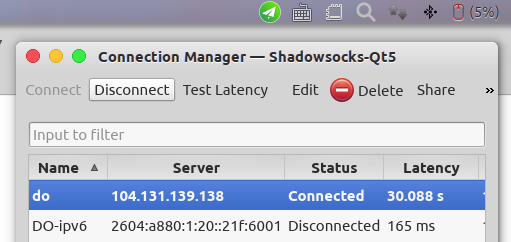
\includegraphics[width=0.4\hsize]{pic/ss客户端.png}
    \centering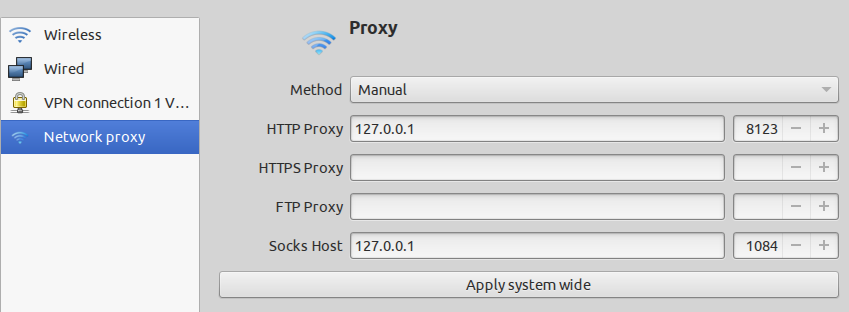
\includegraphics[width=0.45\hsize]{pic/全局代理.png}
\end{frame}


\begin{frame}{免费个人主页 + 个人git私服}
 \begin{block}{}
  个人主页
 \end{block}

 
 \begin{itemize}
  \item \href{https://pages.github.com/}{github pages},部署完成后按 \href{iampkuhz.github.io}{XXXX.github.io} 访问
  \item jekyll + markdown (实际写文件只需要写XXX.md的文件就行,一篇文章一个markdown文本文件,可以嵌套html),排版交给jekyll统一渲染
  \item 可以改域名/访问网址,jekyll项目也可以搭建在VPS上
 \end{itemize}
 
 \begin{block}{}
  \href{http://www.liaoxuefeng.com/wiki/0013739516305929606dd18361248578c67b8067c8c017b000/00137583770360579bc4b458f044ce7afed3df579123eca000}{git私服}
 \end{block}
 \begin{block}{}
  在VPS中\href{https://www.digitalocean.com/community/tutorials/how-to-setup-your-own-vpn-with-pptp}{搭建VPN} (\href{http://yansu.org/2013/12/11/deploy-pptp-vpn-in-ubuntu.html}{一键安装脚本})
 \end{block}
\end{frame}



\section{synergy, JetBrain}
\begin{frame}{synergy, JetBrain}
 \begin{block}{synergy}
  全平台的鼠标、键盘共享软件。只要两台电脑链接同一局域网,就可以使用一套键鼠来在操纵两个电脑
 \end{block}

 \begin{block}{JetBrain家族产品}
  写各个语言的都有:Java(`IntelliJ`), Python(`PyCharm`), php/html(`PhpStorm`),...
  丰富的插件、快捷键;
 \end{block}
\end{frame}

\end{document} 